\documentclass[aspectratio=169]{beamer}
\setbeamertemplate{navigation symbols}{}
\usepackage{color, amsmath, comment, subfigure}
\usepackage{url}
\usepackage{ulem}

\usepackage{hyperref}
\hypersetup{
    colorlinks=true,
    linkcolor=blue,
    filecolor=magenta,      
    urlcolor=cyan,
}

%%%%%%%%%%%%%%%%%%%%%%%%%%
\title[]{Class slides for Thursday, November 5:\\Disease empirics}
\author[]{Matthew J. Salganik}
\institute[]{}
\date[]{COS 597E/SOC 555 Limits to prediction\\Fall 2020, Princeton University}

\begin{document}
%%%%%%%%%%%%%%%%%%%%%%%%%%%
\frame{\titlepage}
%%%%%%%%%%%%%%%%%%%%%%%%%%%
\begin{frame}

\begin{center}
  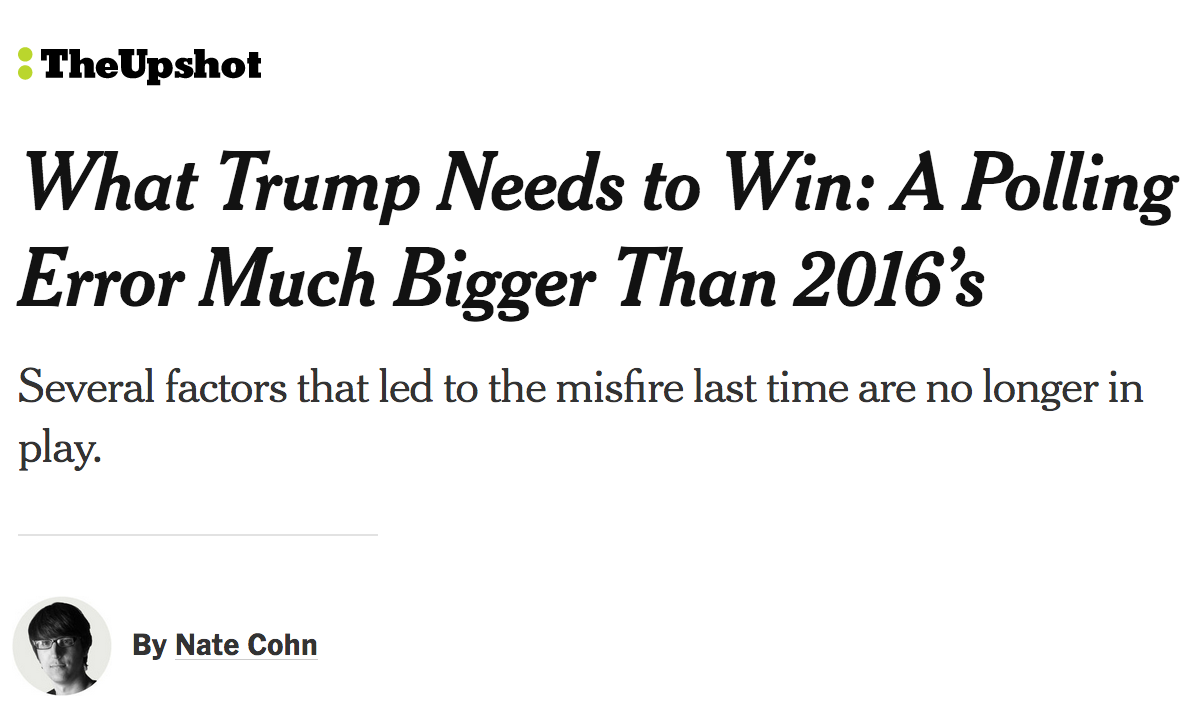
\includegraphics[width = 0.8\textwidth]{figures/cohn_what_2020_title}
\end{center}

\end{frame}
%%%%%%%%%%%%%%%%%%%%%%%%
\begin{frame}

\begin{center}
  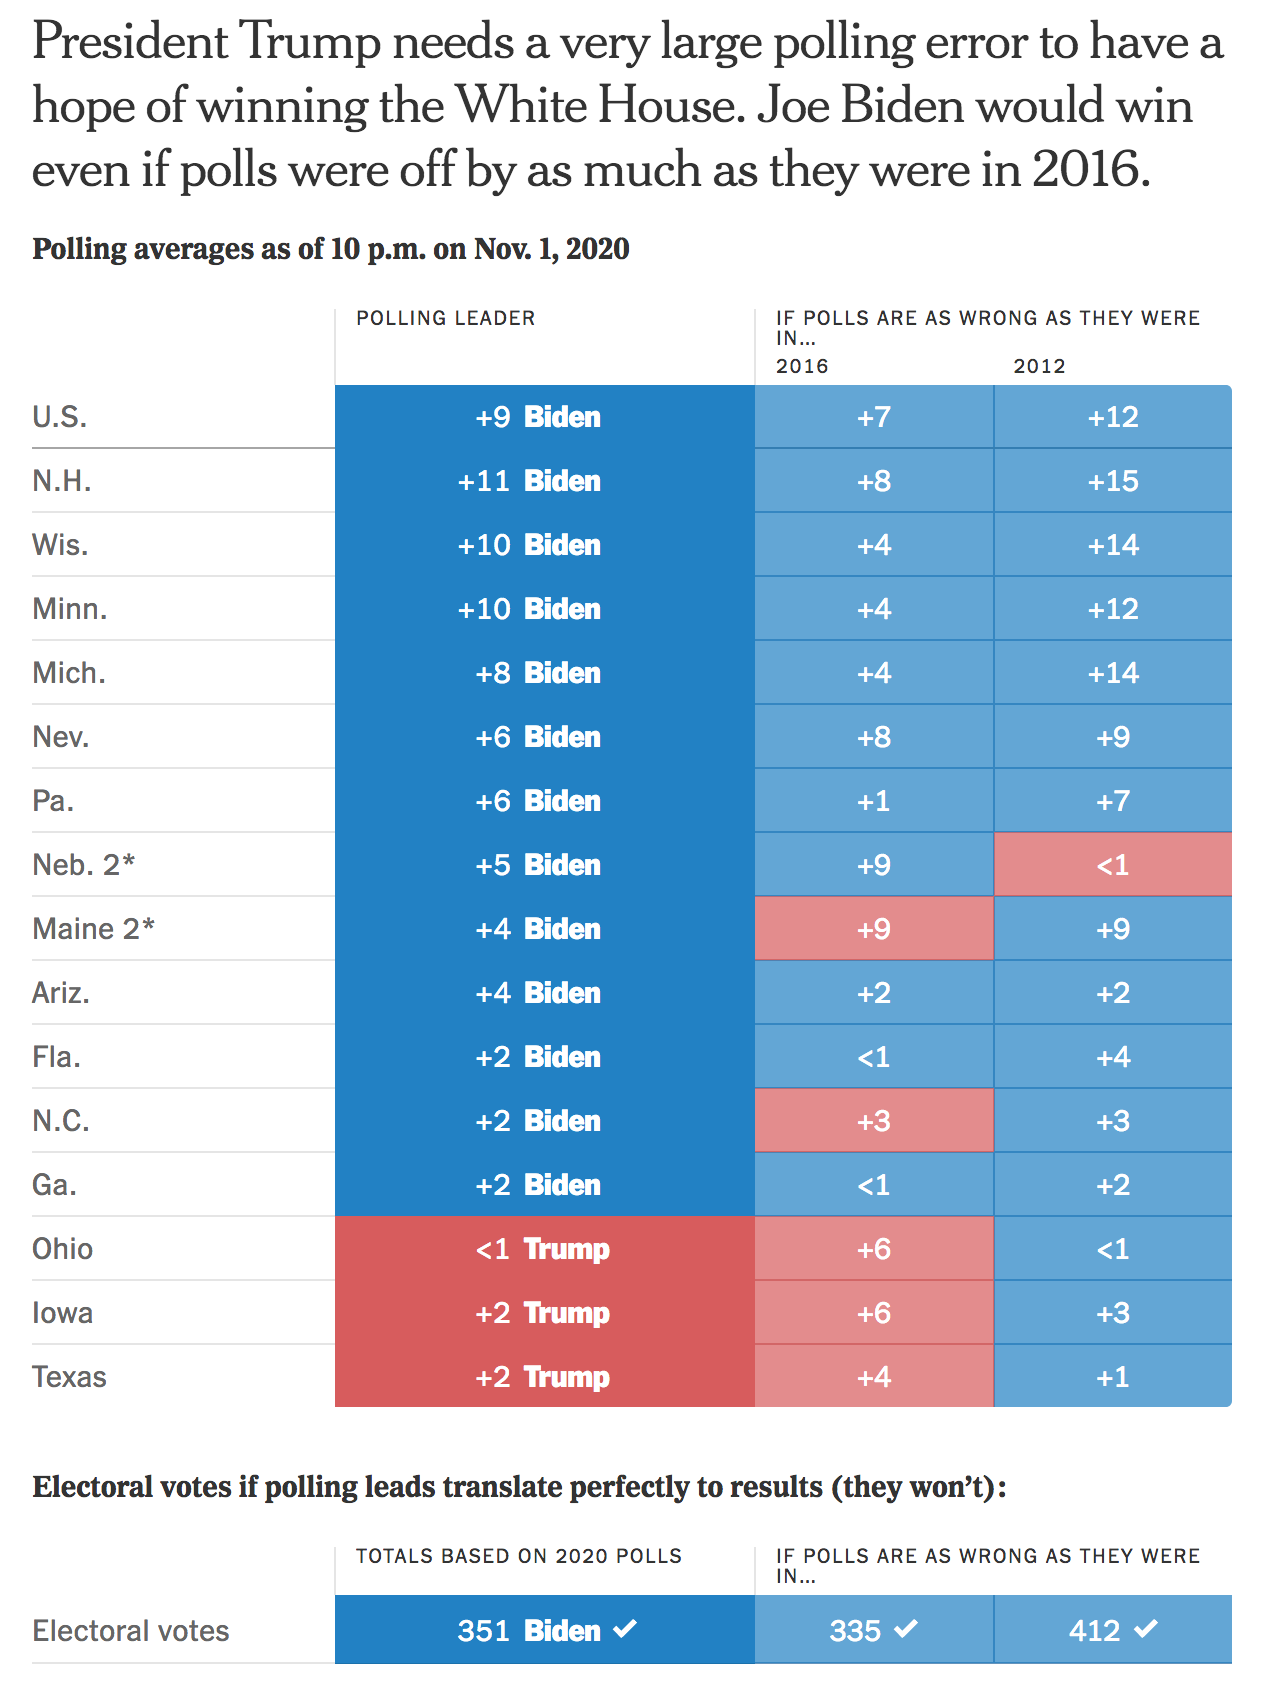
\includegraphics[height = 0.7\textheight]{figures/cohn_what_2020_table}
\end{center}

\pause

Nate Silver: How likely is a big polling error?  We don't have much data. 1948 was biggest poll error on record, but that was different; 2020 is different from 1992.

\vfill
\tiny{\url{https://www.vox.com/21538214/nate-silver-538-2020-forecast-2016-trump-biden-election-podcast}}

\end{frame}
%%%%%%%%%%%%%%%%%%%%%%%%%%%
\begin{frame}

\begin{center}
  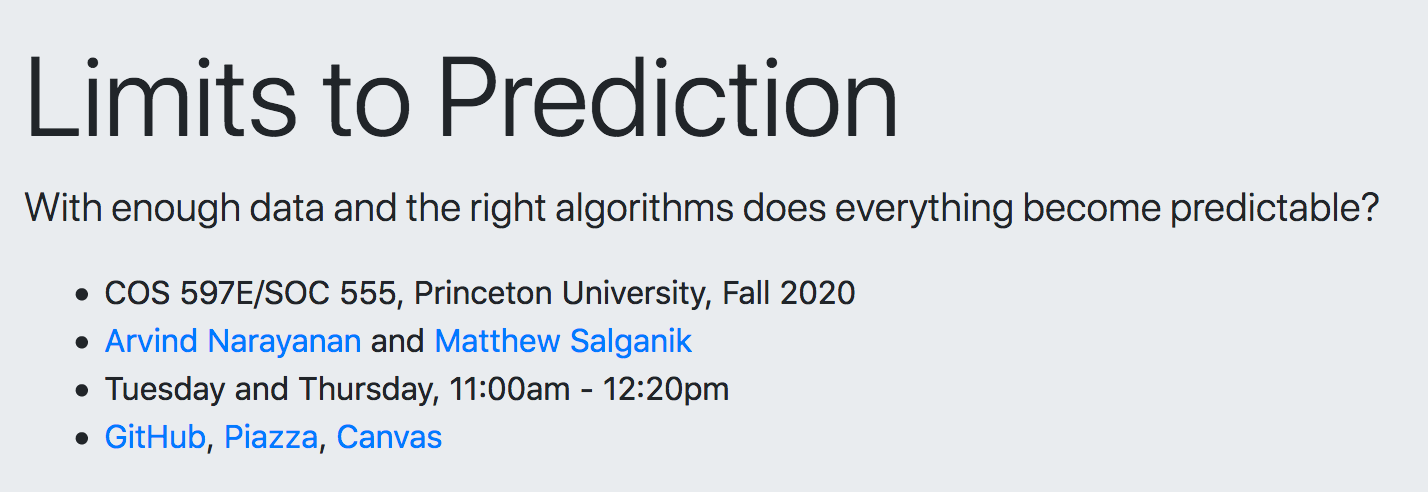
\includegraphics[width = \textwidth]{figures/class_hero}
\end{center}

\end{frame}
%%%%%%%%%%%%%%%%%%%%%%%%
\frame{\titlepage}
%%%%%%%%%%%%%%%%%%%%%%%%%%


\begin{frame}

\begin{center}
  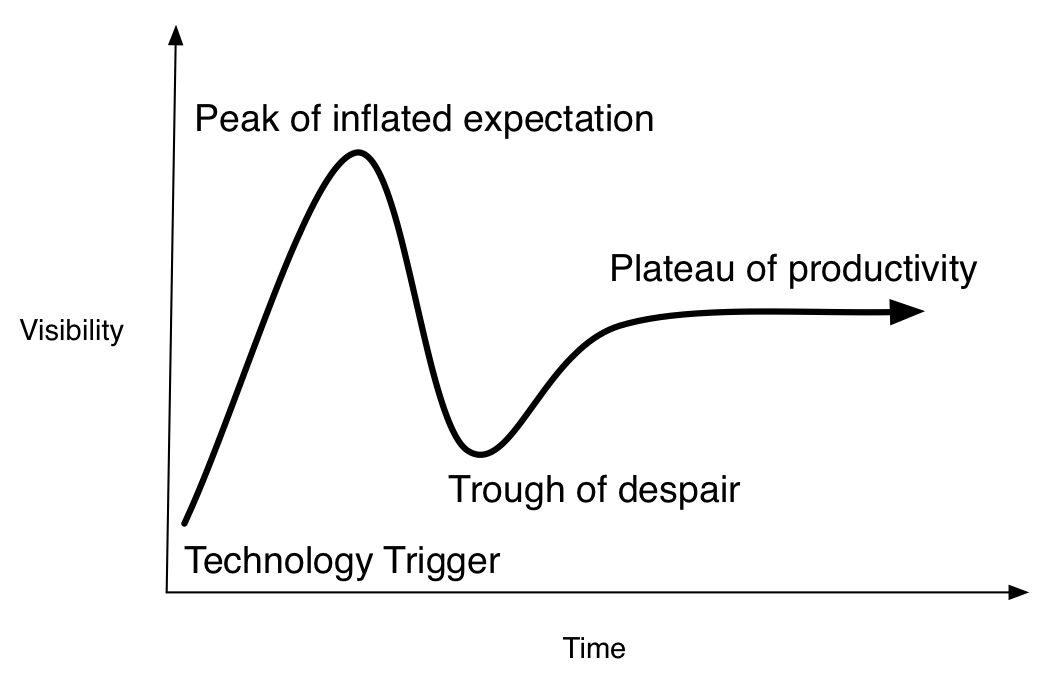
\includegraphics[width = 0.8\textwidth]{figures/hype_cycle}
\end{center}

\vfill
\url{https://en.wikipedia.org/wiki/Hype_cycle}

\end{frame}
%%%%%%%%%%%%%%%%%%%%%%%%%%%%%%%%%
\begin{frame}

\begin{center}
  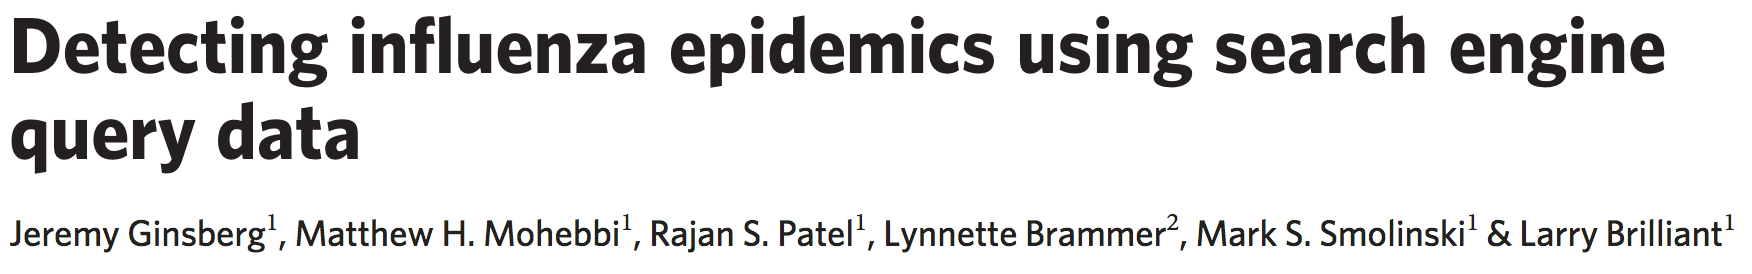
\includegraphics[width = 0.9\textwidth]{figures/ginsberg_detecting_2009_title}
\end{center}

\end{frame}
%%%%%%%%%%%%%%%%%%%%%%%%%%%%%%%%%
\begin{frame}

\begin{center}
  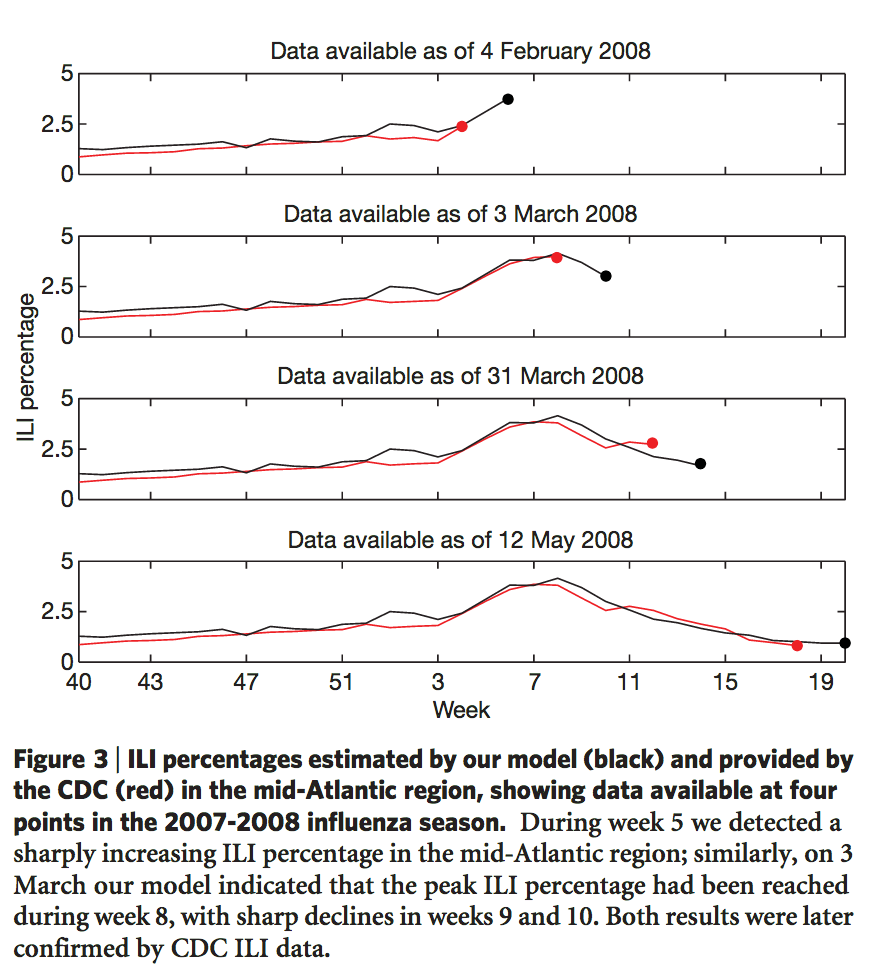
\includegraphics[height = 0.9\textheight]{figures/ginsberg_detecting_2009_fig3}
\end{center}

\end{frame}
%%%%%%%%%%%%%%%%%%%%%%%%%%%%%%%%%%
\begin{frame}

\begin{itemize}
\item Trade-off between manual vs automatic selection of query terms
\pause
\item Very simple model $logit(I(t)) = \alpha logit(Q(t)) + \epsilon$ (where is the magic coming from?)
\pause
\item Performance metric: correlation between CDC and estimates
\pause
\item Using digital trace data to measure/predict other things
\end{itemize}

\end{frame}
%%%%%%%%%%%%%%%%%%%%%%%%%%%%%%%%
\begin{frame}

Lots of hype and a bit of criticism

\end{frame}
%%%%%%%%%%%%%%%%%%%%%%%%%%%%%%%%%
\begin{frame}

\begin{center}
  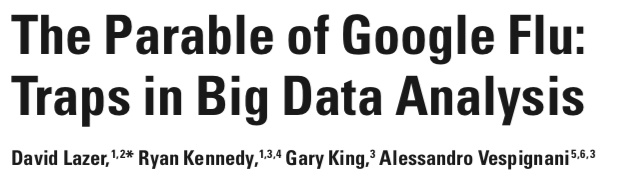
\includegraphics[width = 0.85\textwidth]{figures/lazer_parable_2014_title}
\end{center}

\end{frame}
%%%%%%%%%%%%%%%%%%%%%%%%%%%%%%%%%
\begin{frame}

\begin{center}
  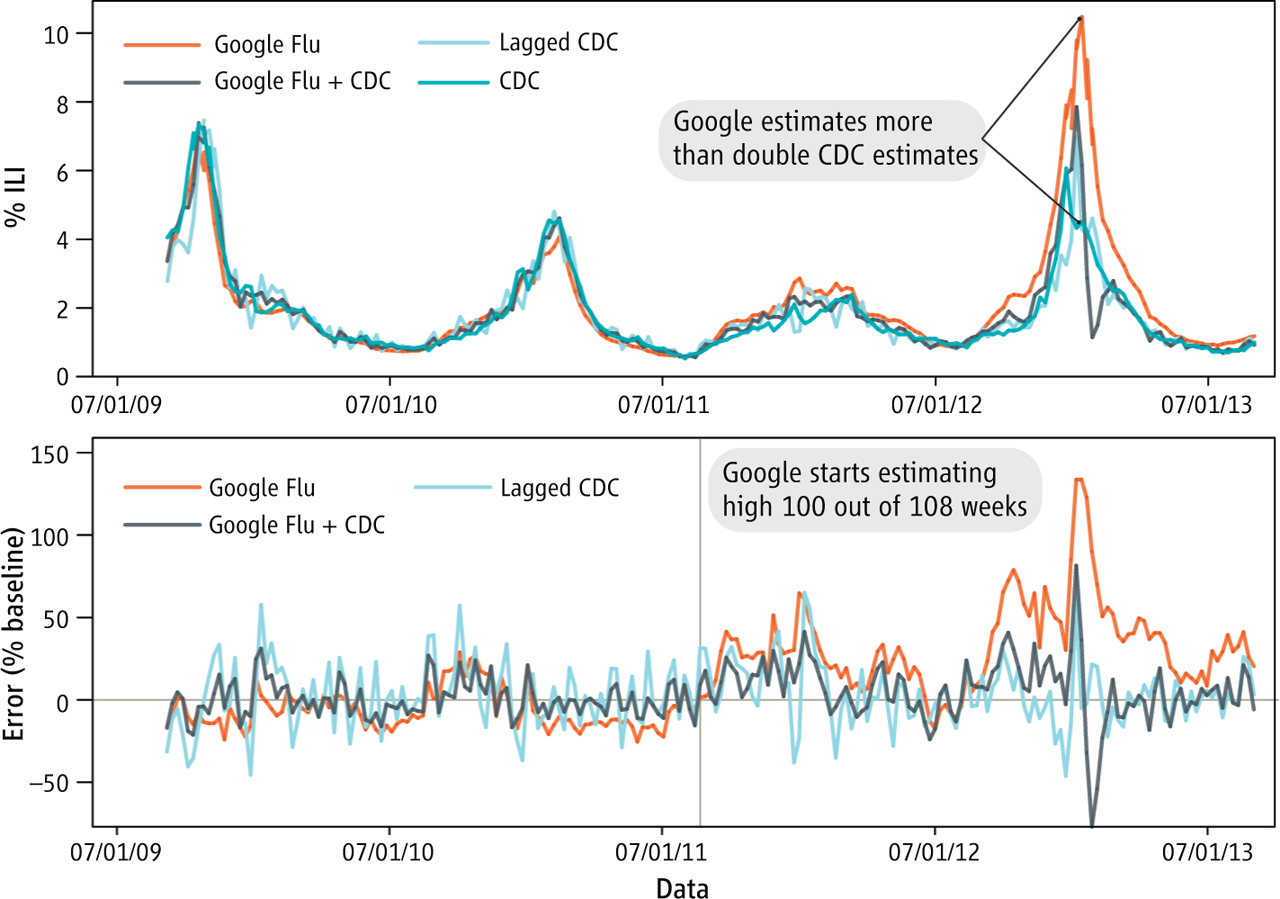
\includegraphics[width = 0.85\textwidth]{figures/lazer_parable_2014_fig2}
\end{center}

\end{frame}
%%%%%%%%%%%%%%%%%%%%%%%%%%%%%%%%%
\begin{frame}

\begin{center}
  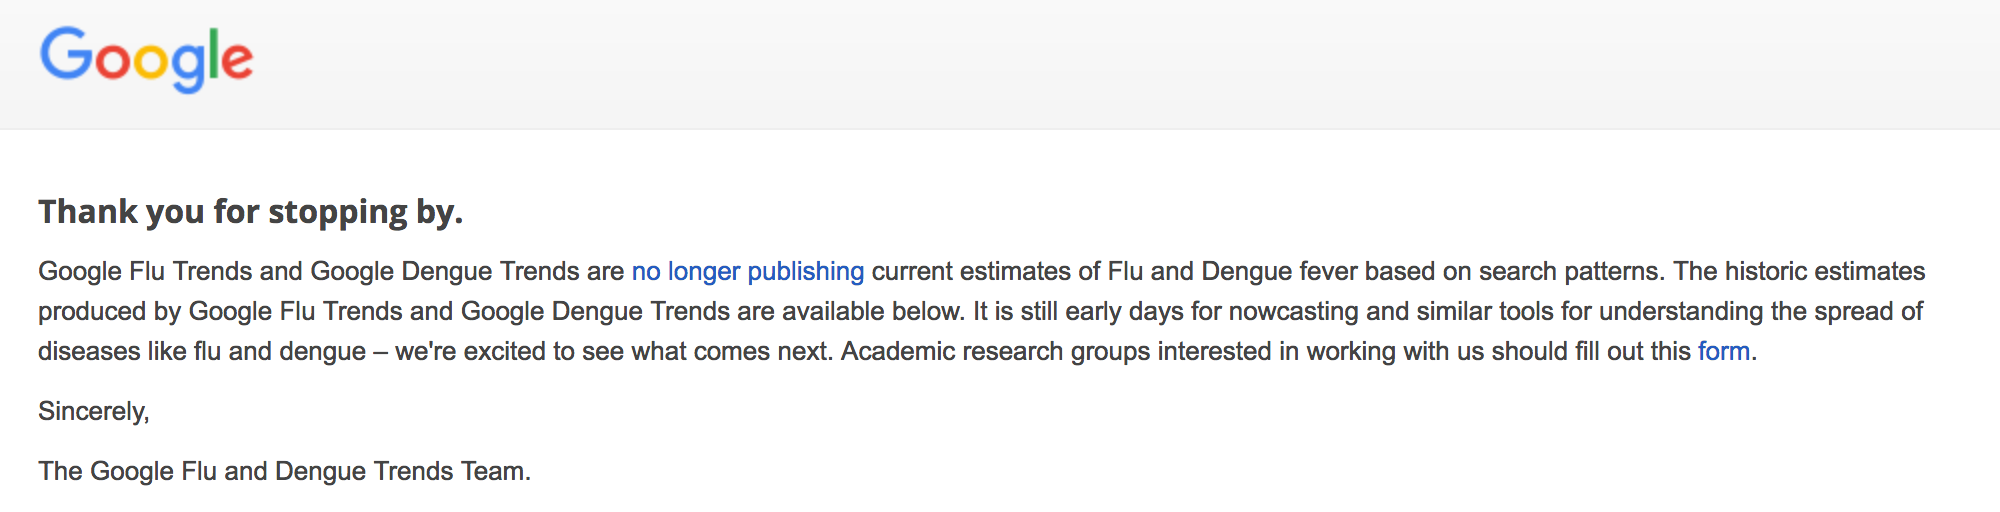
\includegraphics[width = 0.9\textwidth]{figures/google_flu_closed}
\end{center}

\vfill
Nice history: \url{https://www.theatlantic.com/technology/archive/2014/03/in-defense-of-google-flu-trends/359688/}

\end{frame}
%%%%%%%%%%%%%%%%%%%%%%%%%%%%%%%%%%%%%%%%
\begin{frame}

Three lessons from the parable
\begin{itemize}
\item Transparency and replicability
\pause
\item Use big data to understand the unknown (What can Google Flu Trends do beyond speeding up an existing system? Small area estimation)
\pause
\item It is not just about the size of the data
\end{itemize}
\pause
\vfill
Other issue: accountability for Google 

\end{frame}
%%%%%%%%%%%%%%%%%%%%%%%%%%%%%%%%%
\begin{frame}

\begin{center}
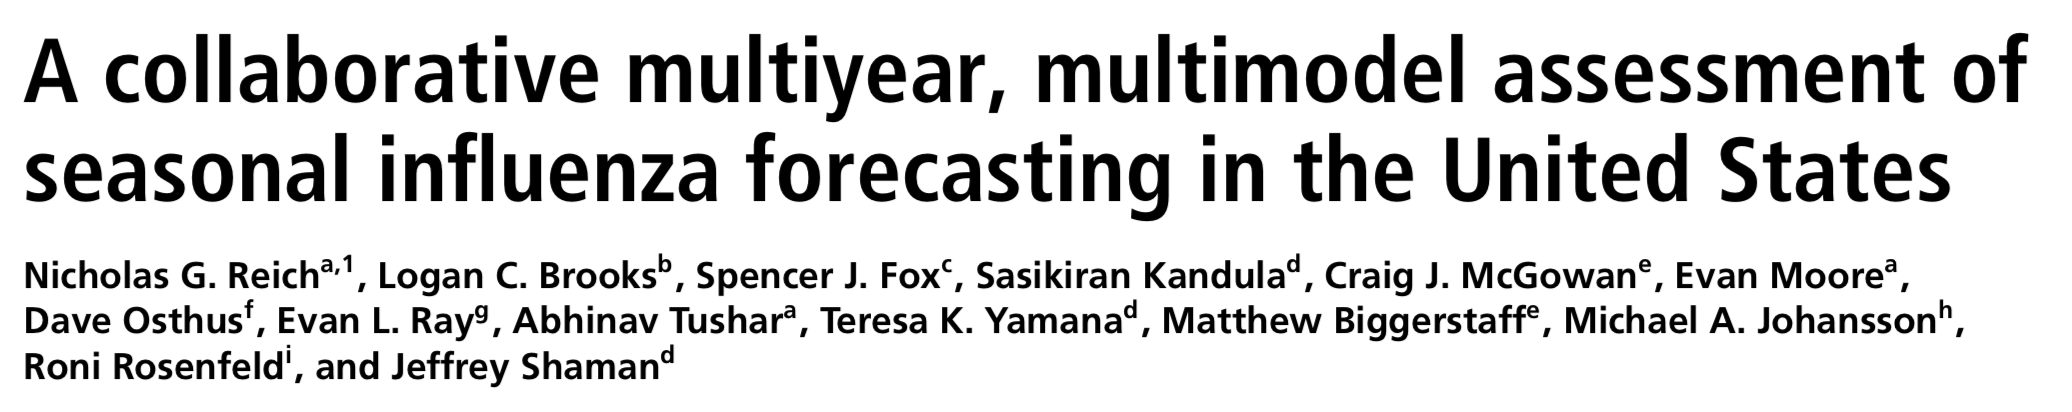
\includegraphics[width = 0.9\textwidth]{figures/reich_collaborative_2019_title}
\end{center}

\end{frame}
%%%%%%%%%%%%%%%%%%%%%%%%%%%%%
\begin{frame}

\begin{itemize}
\item Outcomes related to: \% of patient visits reported through the U.S. Outpatient Influenza-like Illness Surveillance Network (ILINet) were due to influenza-like illness (ILI). 
\pause
\item Target outcomes selected by the CDC, not the researchers
\pause
\item Composite outcome
\end{itemize}

\end{frame}
%%%%%%%%%%%%%%%%%%%%%%%%%%%%%%
\begin{frame}

\begin{center}
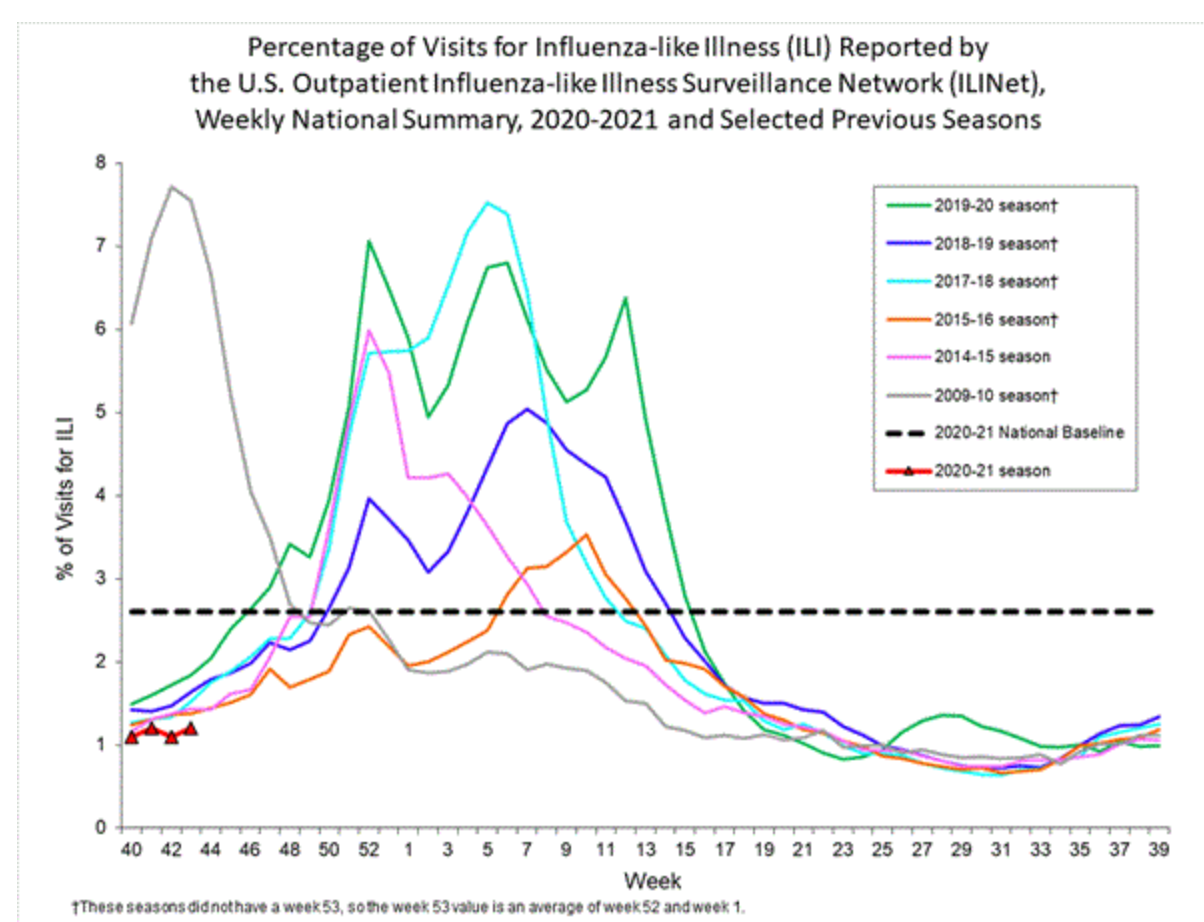
\includegraphics[width = 0.7\textwidth]{figures/ilinet_week43}
\end{center}

\vfill
\url{https://www.cdc.gov/flu/weekly/index.htm\#ILINet}

\end{frame}
%%%%%%%%%%%%%%%%%%%%%%%%%%
\begin{frame}

\begin{center}
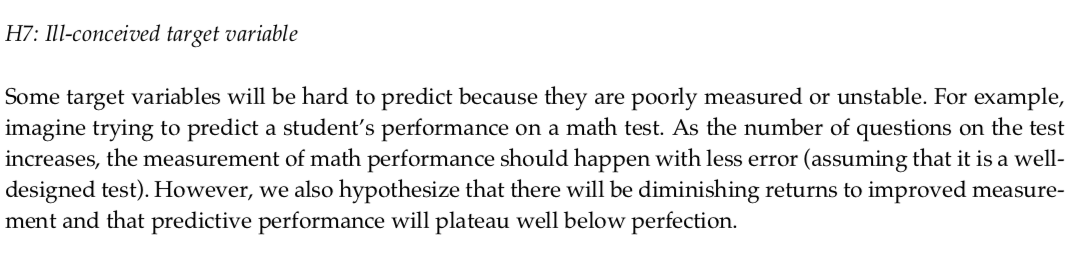
\includegraphics[width = 0.9\textwidth]{figures/preread_outcome}
\end{center}

\vfill 
Please put other composite outcomes in the chat

\end{frame}
%%%%%%%%%%%%%%%%%%%%%%%%%%%
\begin{frame}

\begin{center}
\only<1>{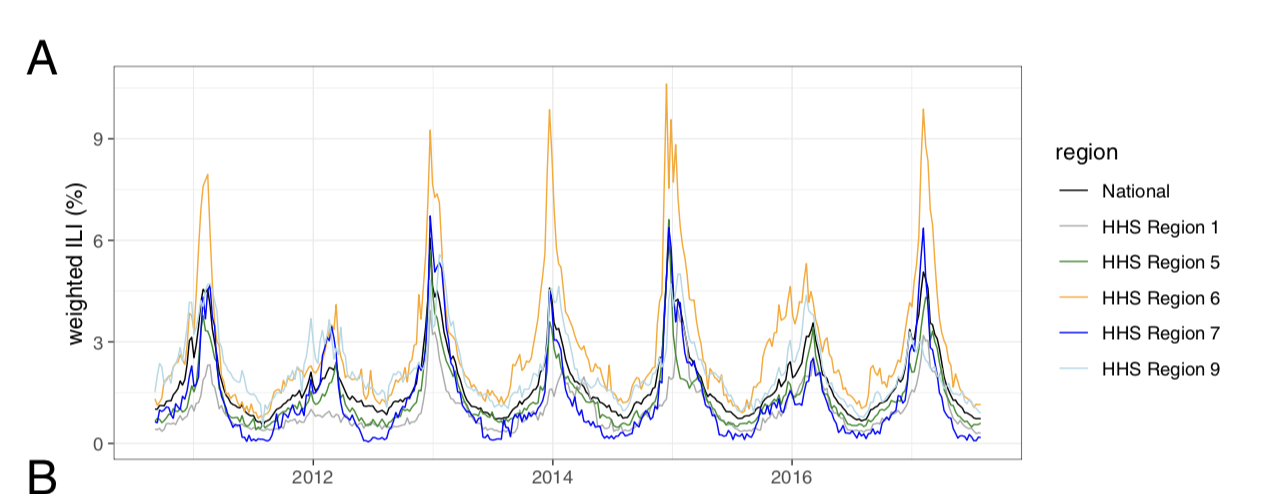
\includegraphics[width = 0.7\textwidth]{figures/reich_collaborative_2019_fig1a}} %
\only<1>{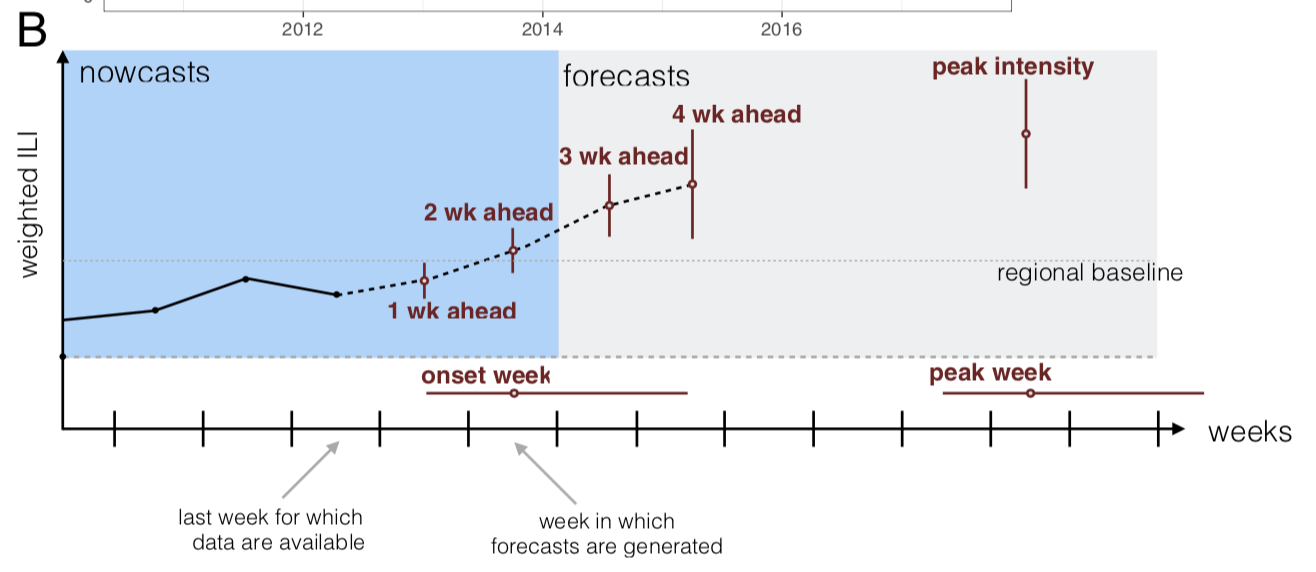
\includegraphics[width = 0.7\textwidth]{figures/reich_collaborative_2019_fig1b}} %
\end{center}

\end{frame}
%%%%%%%%%%%%%%%%%%%%%%%%%%%%%
\begin{frame}

Predictability for a target can be broken into two components: 1) baseline from historical average 2) improvement over baseline. (prediction vs skillful prediction) 

\pause
\begin{center}
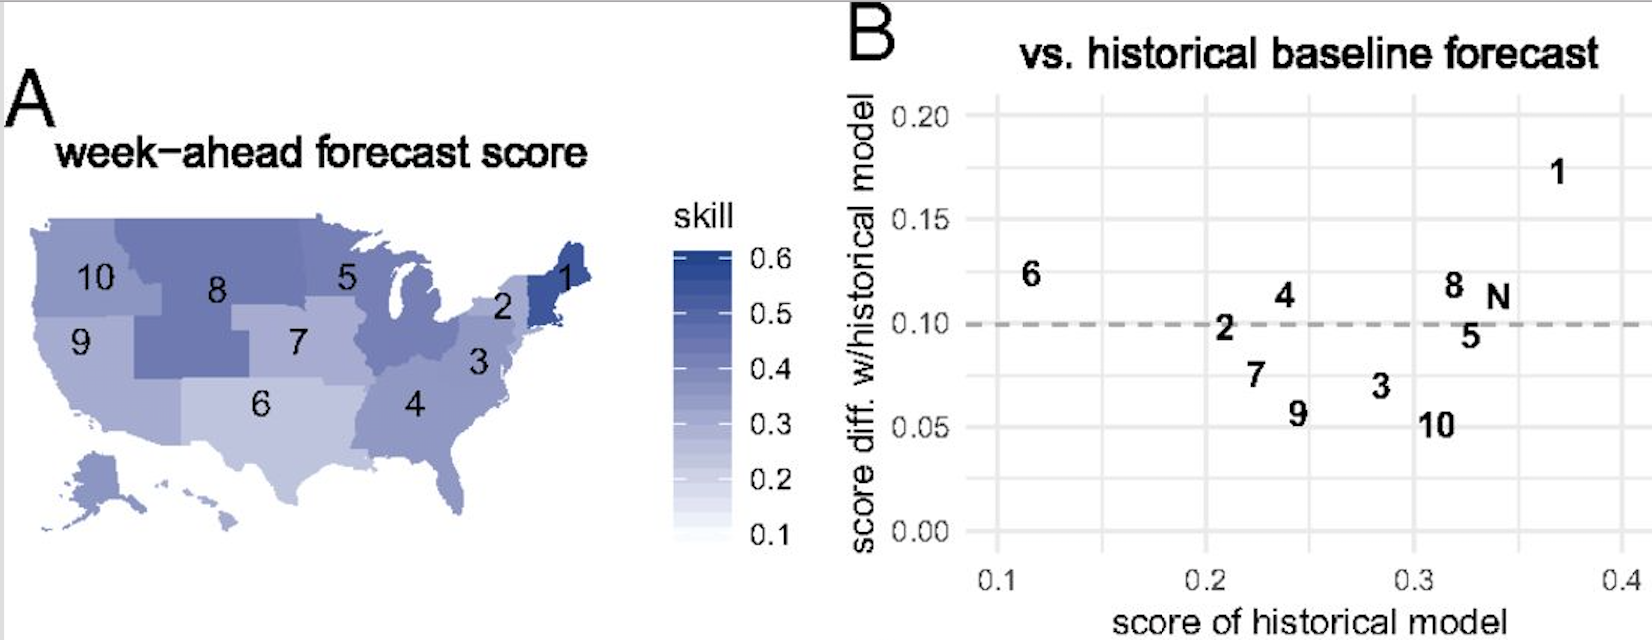
\includegraphics[width = 0.9\textwidth]{figures/reich_collaborative_2019_fig3ab}
\end{center}

\end{frame}
%%%%%%%%%%%%%%%%%%%%%%%%%%%%
\begin{frame}

\begin{center}
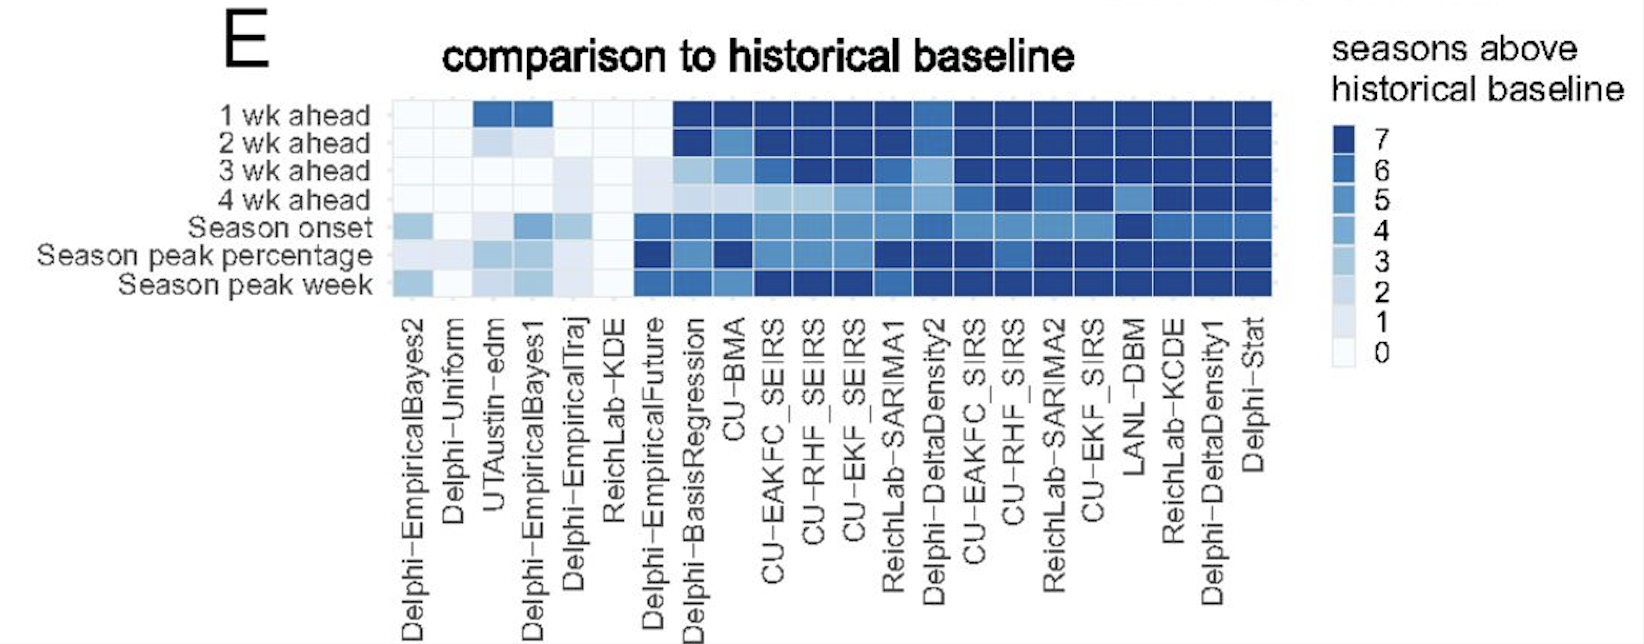
\includegraphics[width = 0.9\textwidth]{figures/reich_collaborative_2019_fig3e}
\end{center}

Doing better than historical baseline is not easy

\end{frame}
%%%%%%%%%%%%%%%%%%%%%%%%%%%%
\begin{frame}

How does forecast score decay as time window increases? \pause \\
\texttt{CU-EKF\_SIRS} (best): 0.55 (1 week ahead), 0.44 (2 weeks ahead), 0.36 (3 weeks ahead), 0.31 (4 weeks ahead)

\end{frame}
%%%%%%%%%%%%%%%%%%%%%%%%%%%%
\begin{frame}

Scores were lower for seasonal targets than week-ahead targets, although model showed greater relative improvement compared to baseline.  In other words, it the details of the outcome matter.

\end{frame}
%%%%%%%%%%%%%%%%%
\begin{frame}

\begin{center}
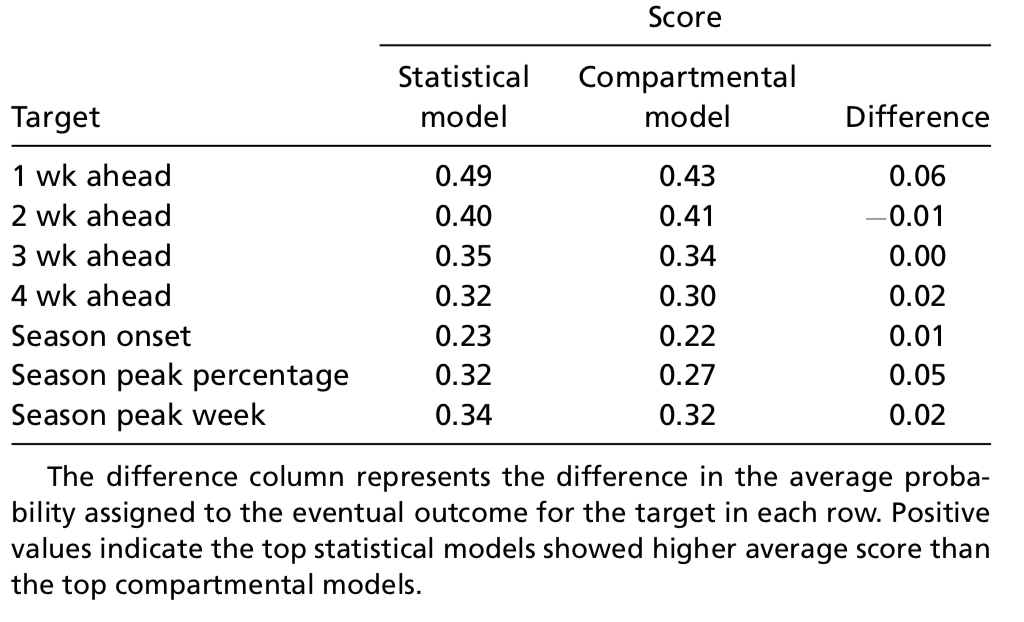
\includegraphics[width = 0.7\textwidth]{figures/reich_collaborative_2019_tab2}
\end{center}

\vfill
\begin{itemize}
\item Compartmental model
\pause 
\item Value of the multiple analyst design
\pause
\item Can we quantify the value of the multiple analyst design?
\end{itemize}

\end{frame}
%%%%%%%%%%%%%%%%%%%%%%%%%%%%%
\begin{frame}

\begin{center}
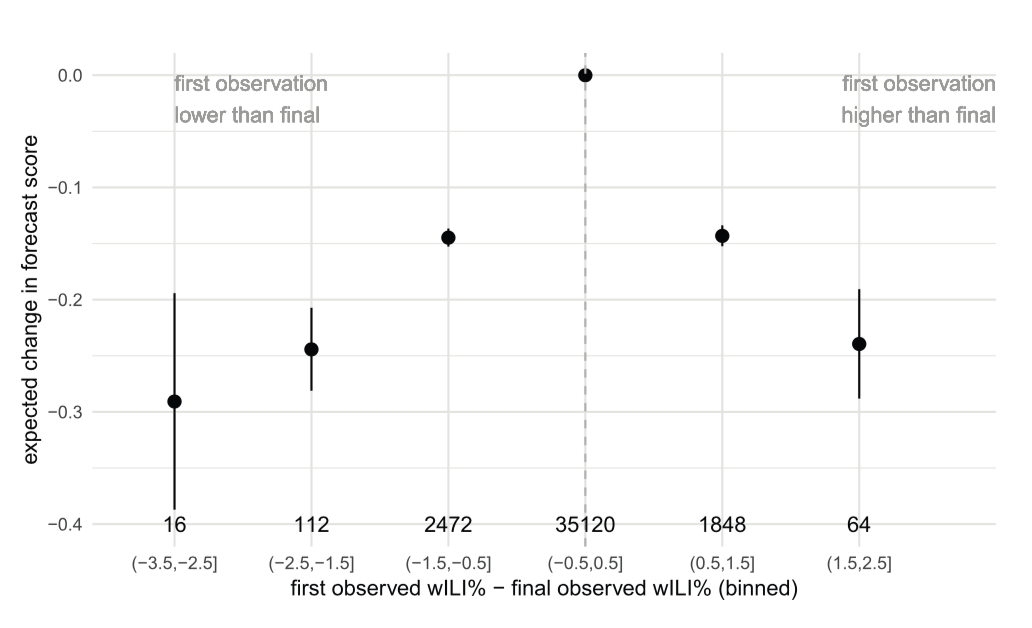
\includegraphics[width = 0.7\textwidth]{figures/reich_collaborative_2019_fig6}
\end{center}

Bad initial measurements hurt performance. Measuring the present helps us predict the future

\end{frame}
%%%%%%%%%%%%%%%%%%%%%%%%%%%%%
\begin{frame}

\begin{center}

\includegraphics[width = 0.9\textwidth]{figures/bracher_on_2019_title}
\end{center}

\begin{itemize}
\item proper scoring rules encourage accurate reporting, but how important is that here?
\pause
\item important question for the design of prediction tasks
\end{itemize}

\end{frame}
%%%%%%%%%%%%%%%%%%%%%%%%%%%
\begin{frame}

\begin{center}
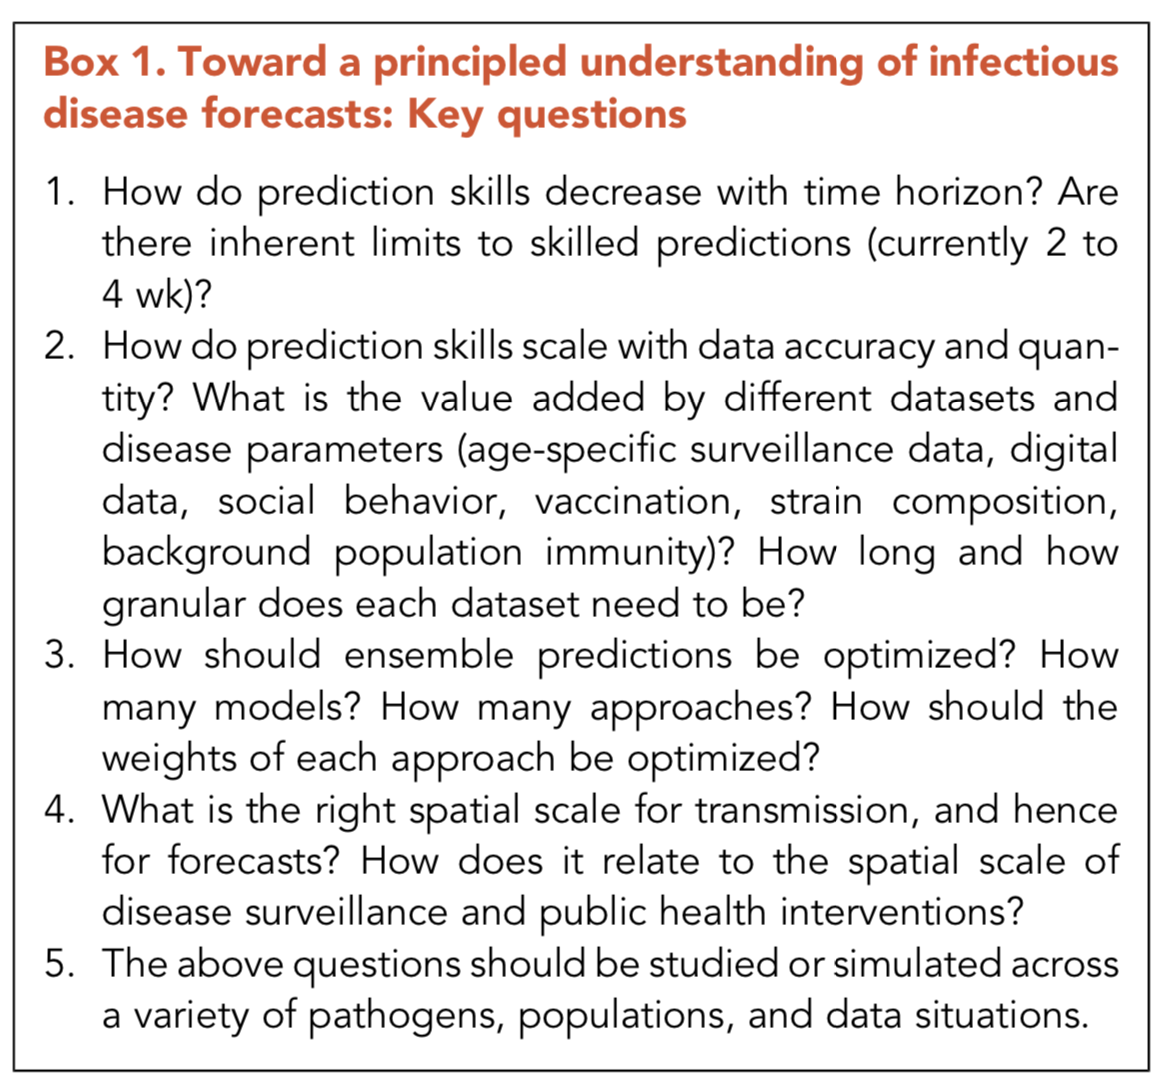
\includegraphics[height = 0.9\textheight]{figures/viboud_future_2019_box1}
\end{center}

\end{frame}
%%%%%%%%%%%%%%%%%%%%%%%%%%%%%
\begin{frame}

\begin{center}
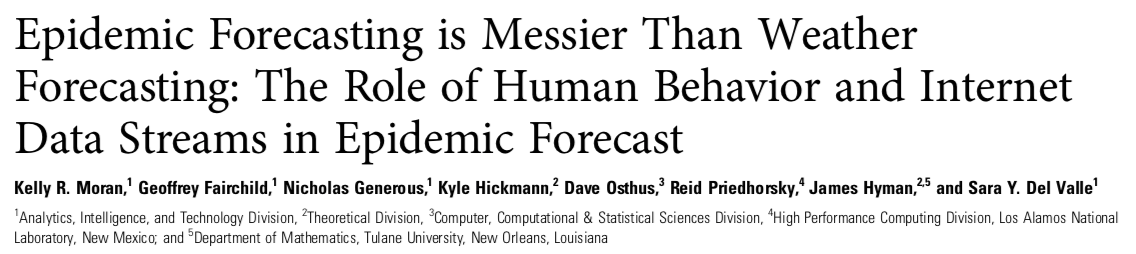
\includegraphics[width = 0.9\textwidth]{figures/moran_epidemic_2016_title}
\end{center}

\end{frame}
%%%%%%%%%%%%%%%%%%%%%%%%%%%%%
\begin{frame}

\begin{center}
Data access
\end{center}

\end{frame}
%%%%%%%%%%%%%%%%%%%%%%%%%%%%%%%%%%%%%%%%
\begin{frame}

\begin{center}
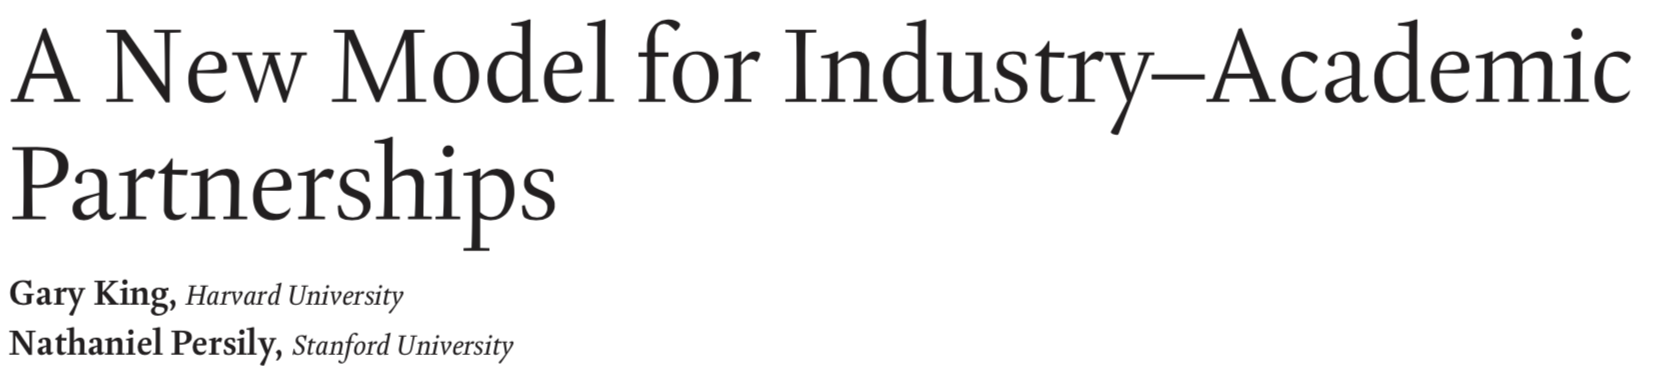
\includegraphics[width = 0.9\textwidth]{figures/king_new_2020_title}
\end{center}

\end{frame}
%%%%%%%%%%%%%%%%%%%%%%%%%%%%%%%%%%%%%%%%
\begin{frame}

\begin{center}
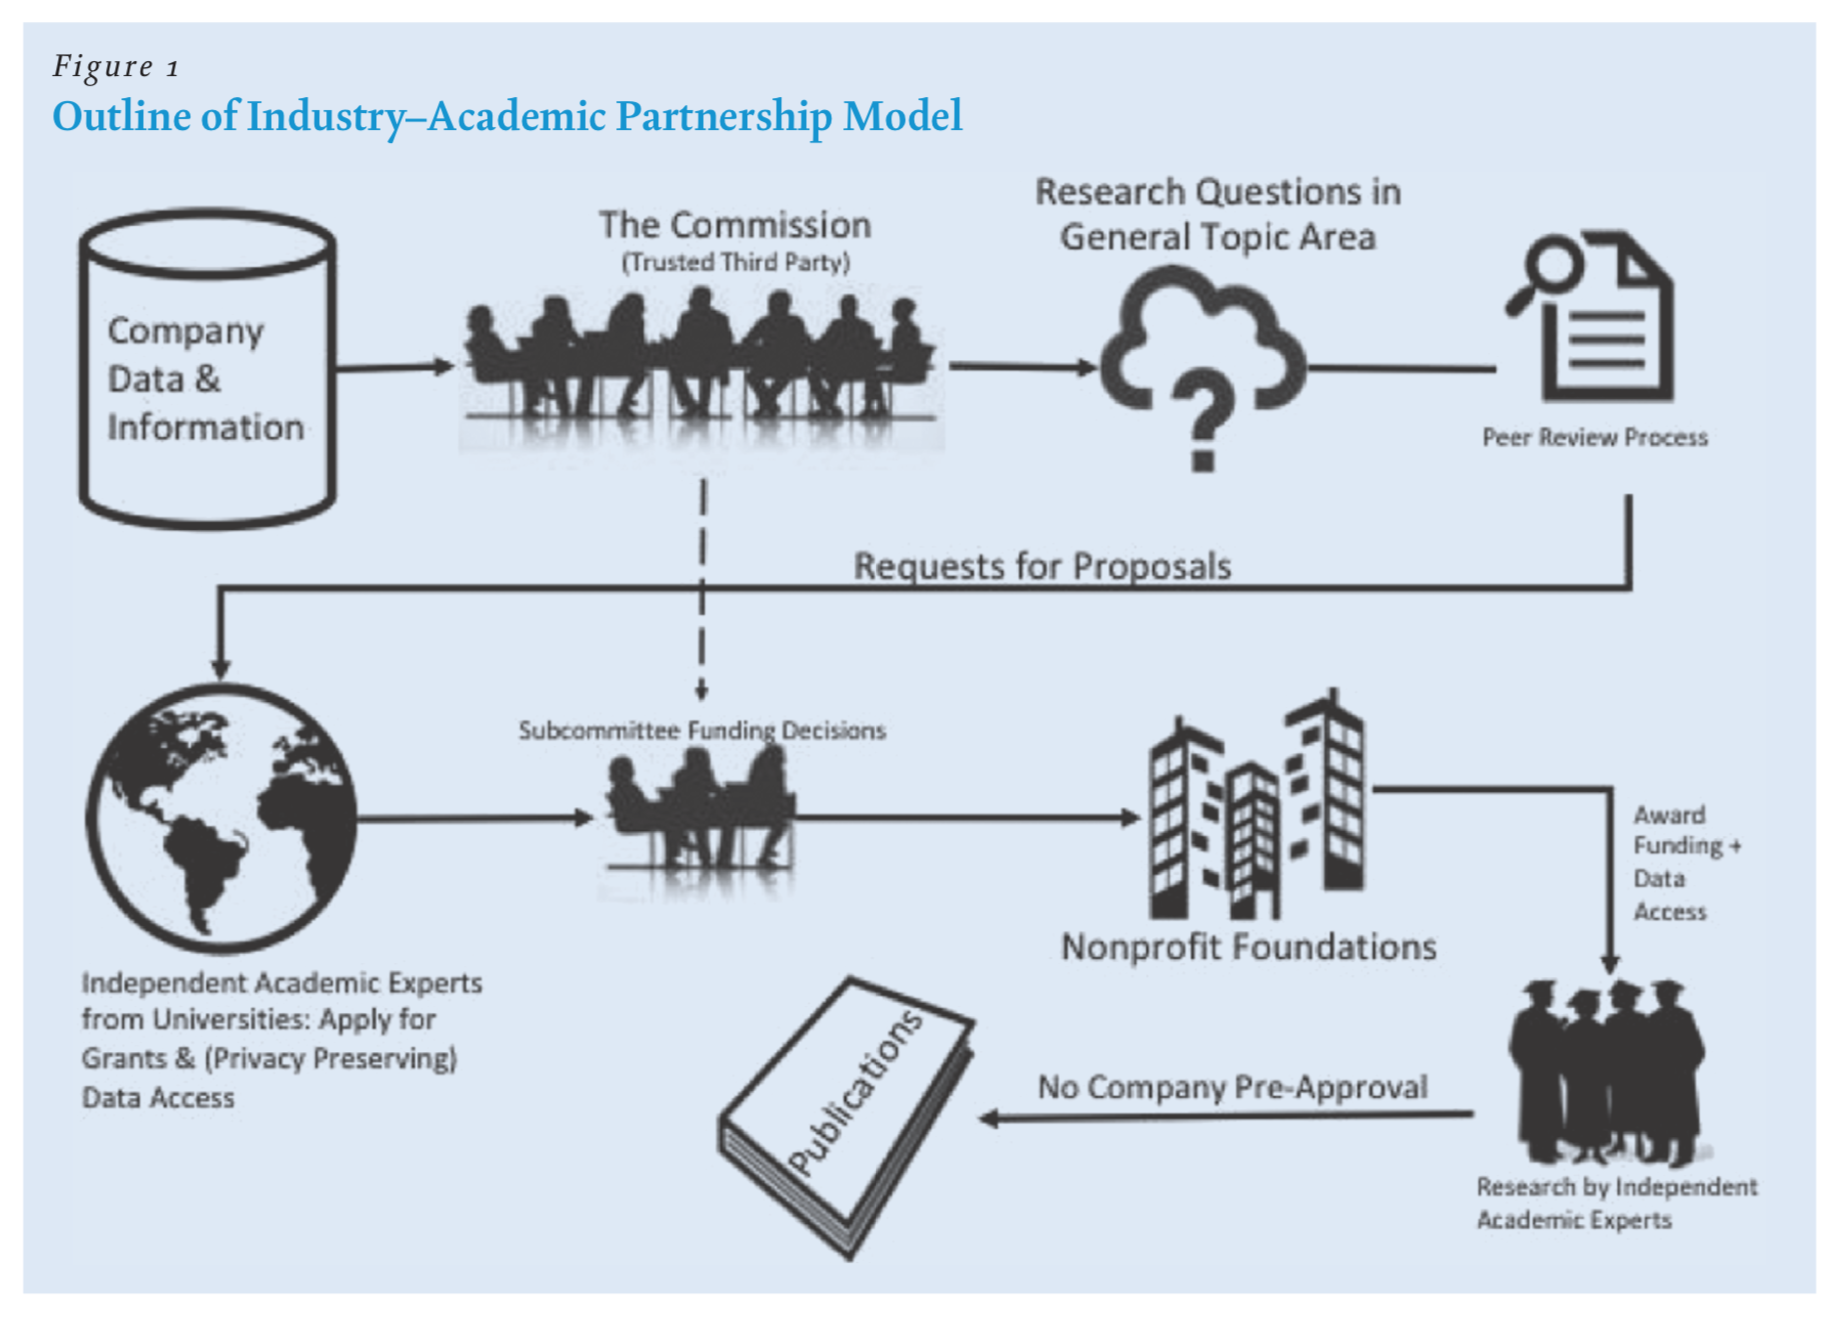
\includegraphics[width = 0.8\textwidth]{figures/king_new_2020_fig1}
\end{center}

\end{frame}
%%%%%%%%%%%%%%%%%%%%%%%%%%%%%%%%%%%%%%%%
\begin{frame}

My 3 takeaways:
\begin{itemize}
\item Data access as a limit to prediction
\pause
\item Composite outcomes as a limit to prediction (prevents isolation of one system)
\pause
\item How much data do we really have?
\end{itemize}

\end{frame}
%%%%%%%%%%%%%%%%%%%%%%%%%%
\begin{frame}

Split into groups

\end{frame}
%%%%%%%%%%%%%%%%%%%%%%%%%%
\begin{frame}

\tiny{
\begin{tabular}{ccc}
\hline
 & Weather & Disease\\
\hline
Knowledge of fund laws \pause & high & high for medical, low for social \pause \\ 
Global cooperation \pause & Possible & creepy (\& potentially dangerous)  \pause \\
Openness of inp, pred \& outs \pause & Public \& standardized & problems from gov (interference) \& firms (inaccessible, bad measurement) \pause \\ 
Reactivity to predictions \pause & Low & Some from people, gov, firms  \pause \\
Adjust to phenomena \pause & None & Some from people, gov, firms \pause \\ 
Goal \pause & Prediction for accommodation & Prediction for intervention \pause \\ 
\hline
\end{tabular}
}

\end{frame}
%%%%%%%%%%%%%%%%%%%%%%%%%%
\begin{frame}

\begin{center}
Provocation:  For weather forecasting fundamental limits come from nature, and for disease forecasting fundamental limits comes from social organization
\end{center}

\end{frame}
%%%%%%%%%%%%%%%%%%%%%%%%%%
\begin{frame}

\begin{columns}

\begin{column}{0.5\textwidth}
\begin{center}
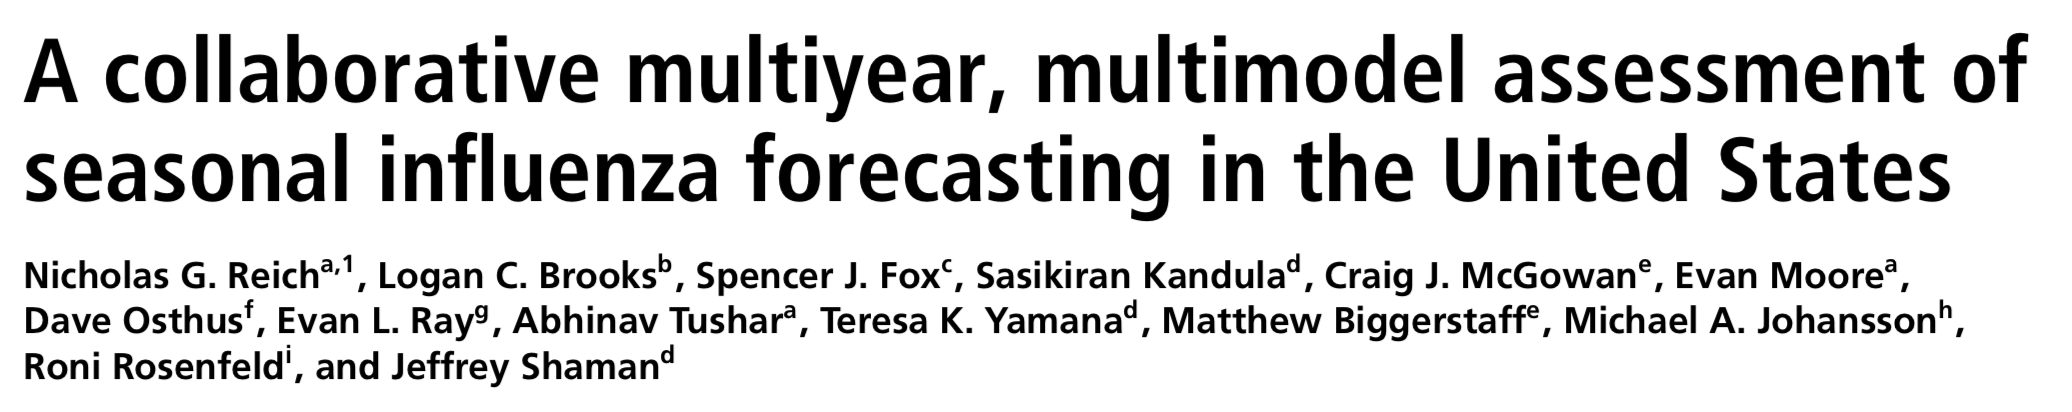
\includegraphics[width = 0.9\textwidth]{figures/reich_collaborative_2019_title}
\end{center}
\end{column}

\pause

\begin{column}{0.5\textwidth}
\begin{center}

\includegraphics[height = 0.8\textheight]{figures/federal_weather_2019}
\end{center}
\vfill
Total budget about 4 billion USD\\
\url{https://www.ofcm.gov/publications/fedrep/2019\_fedrep.pdf}
\end{column}
\end{columns}

\end{frame}
%%%%%%%%%%%%%%%%%%%%%%%%%%
\begin{frame}

\begin{center}
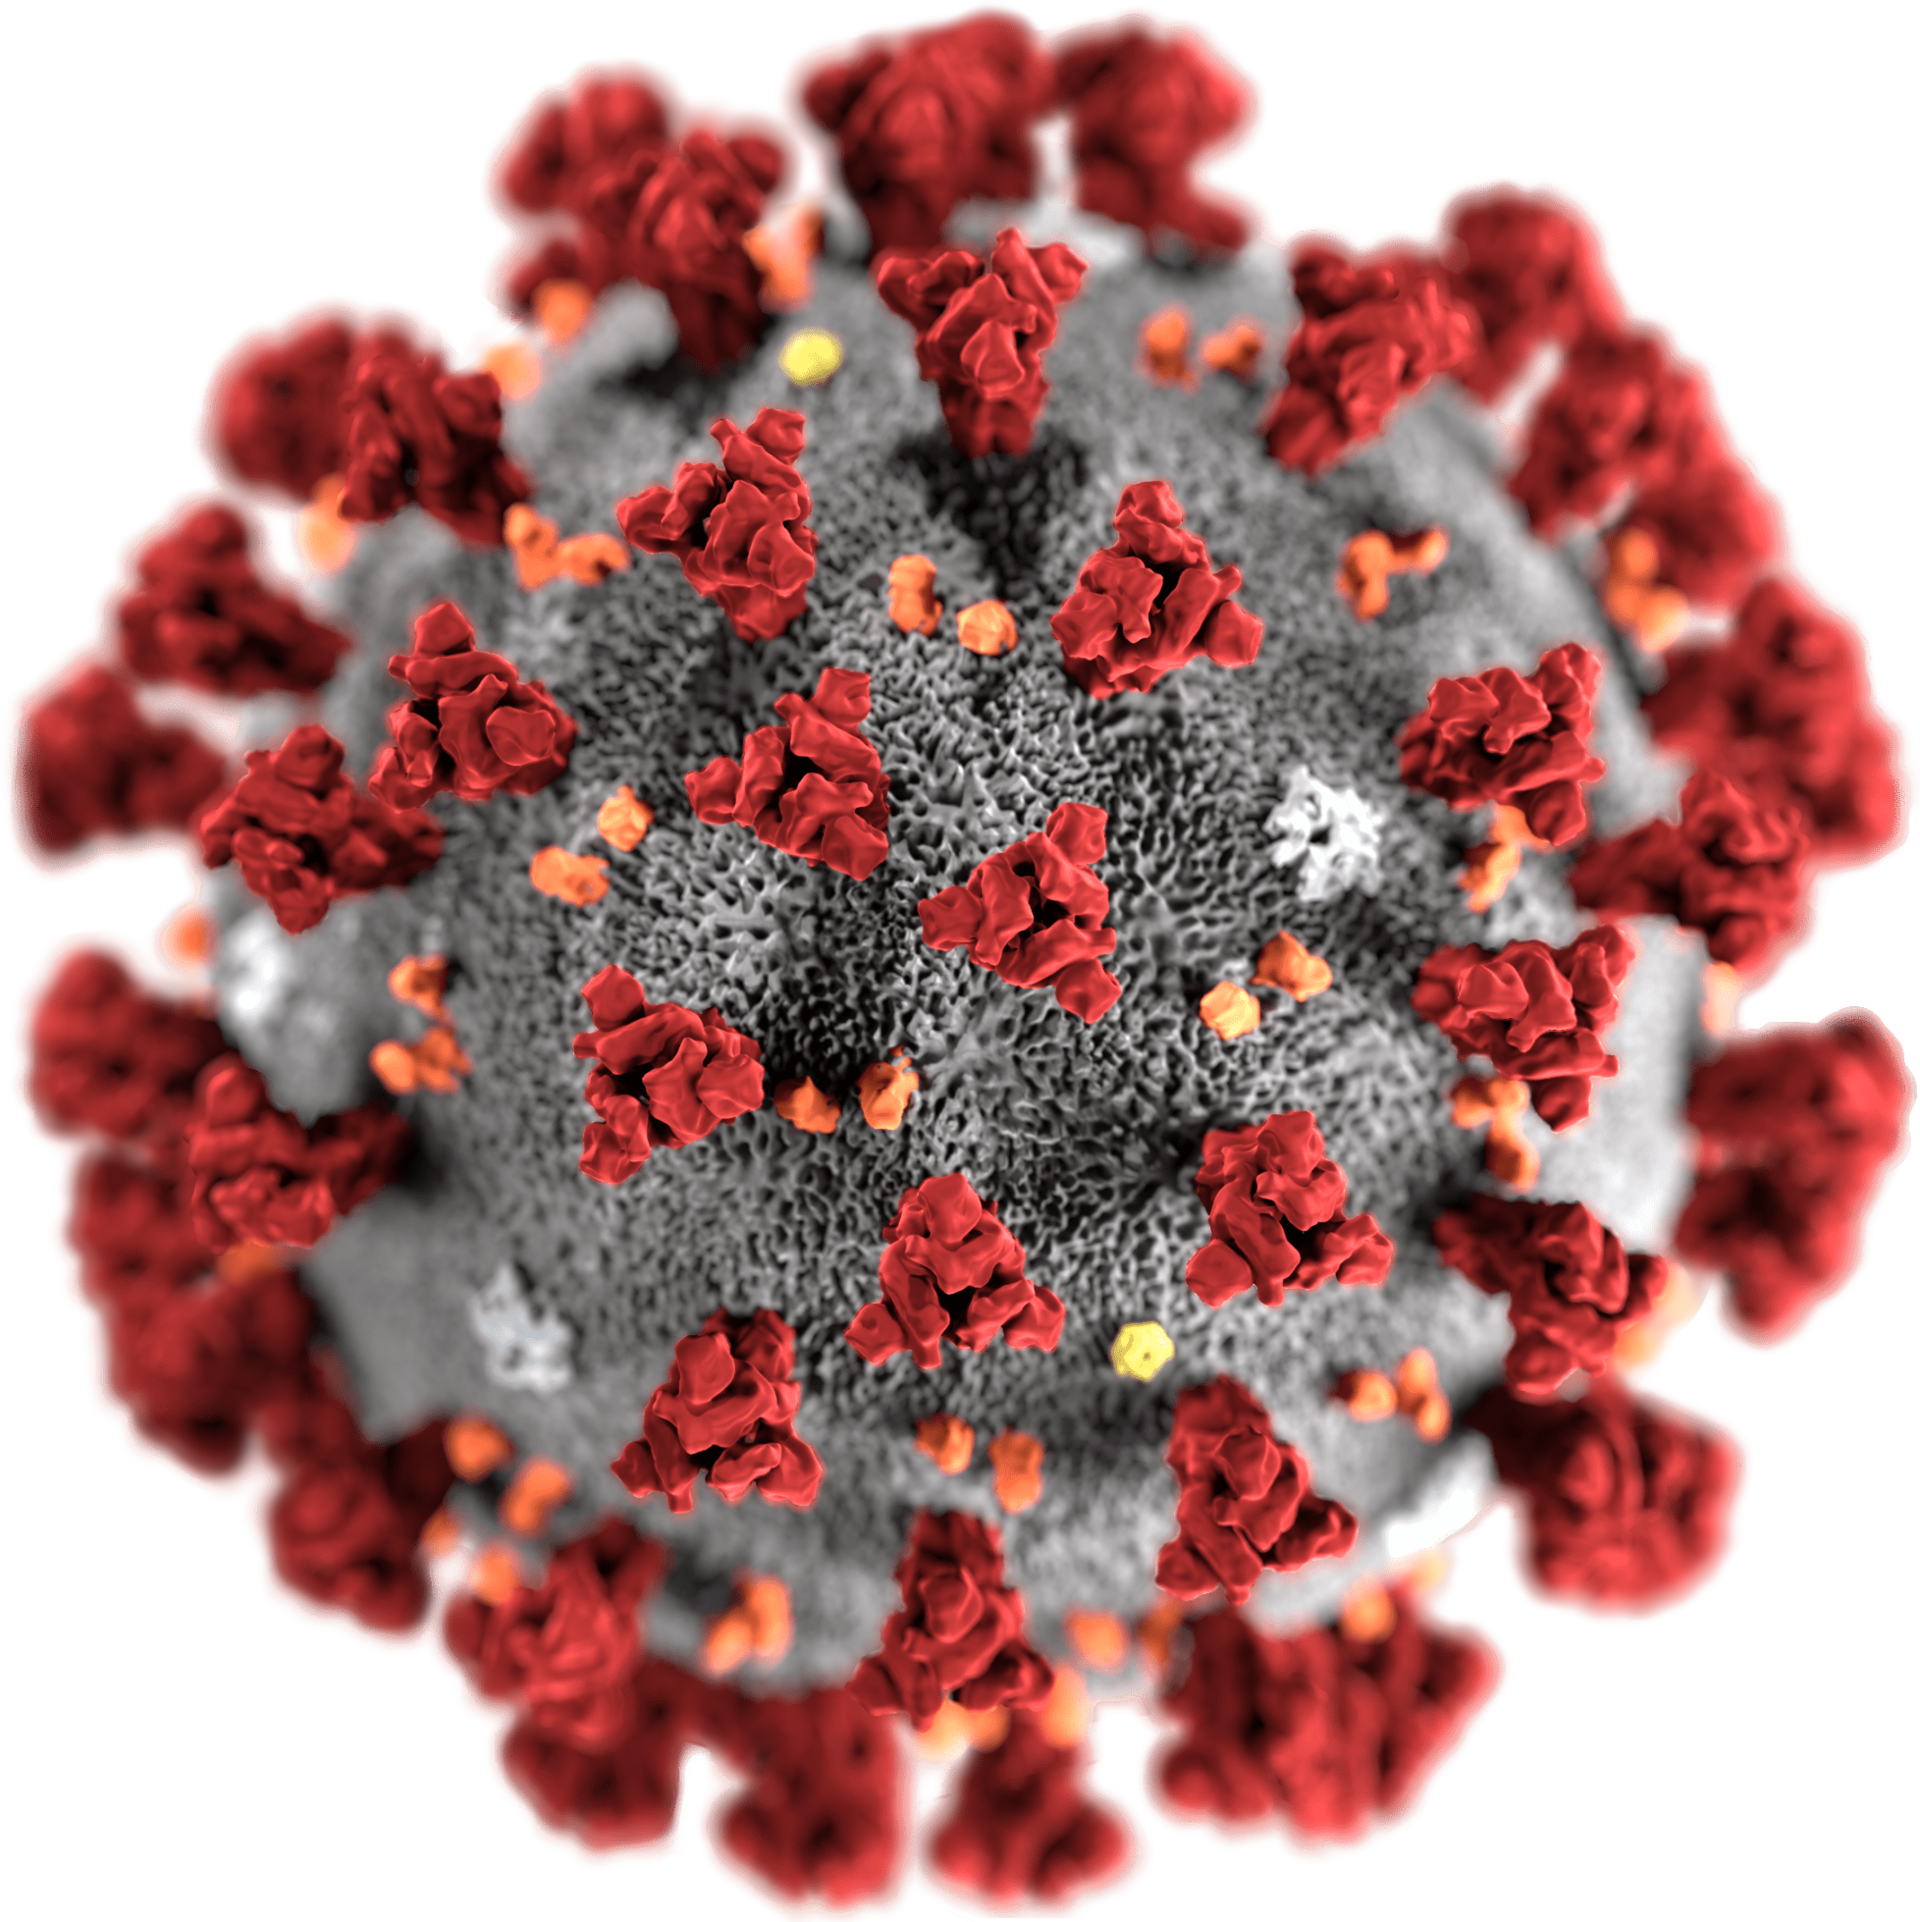
\includegraphics[height = 0.9\textheight]{figures/covid}
\end{center}

\vfill
\tiny{\url{https://phil.cdc.gov/Details.aspx?pid=23312}}
\end{frame}
%%%%%%%%%%%%%%%%%%%%%%%%%%%%
\begin{frame}

Next steps: Predictability of life trajectories
\begin{itemize}
\item Tuesday: Fragile Families Challenge (little reading)
\item Thursday: ``Dark matter'' interviews (lots of reading, potentially emotionally difficult)
\end{itemize}

Send me your completed and signed data agreement by today (Thursday) at 5pm

\end{frame}
%%%%%%%%%%%%%%%%%%%%%%%%%%%%

\frame{\titlepage}


\end{document}
